% !TEX root = main.tex
\section{Experiments and Results}


\begin{table}[t]
    \begin{center}
    \setlength{\tabcolsep}{1.3mm}
\begin{tabular}{r|cccccccccc}
\hline
& {\bf PDIA } & PDIA-MAP & PDIA-$\beta=0$ & HMM & 2-gram& 3-gram & 4-gram & 5-gram & 6-gram & SSM \\
\hline
AIWS & 2.25* & 2.64* & 2.25* & 2.98 & 3.275 & 2.687 & 2.358 & 2.263 & 2.230 & 2.257 \\
AIWS & 205.1* & 212* & 203.8* & 52 & 28 & 382 & 2023 & 5592 & 10838 & 19358 \\
\hline
\hline
AIWL & 2.25* & 2.64* & 2.25* & 2.98 & ? & 2.517 & 2.018 & 1.811 & 1.729 & 1.697 \\
AIWL & 205.1* & 212* & 203.8* & 52 & 28 & 444 & 3249 & 12324 & 31990 & 177232 \\
\hline
\hline
DNA & 1.893* & 1.906* & 1.893* & 1.909* & 1.915* & 1.908* & 1.905* & 1.903* & 1.910* & 1.832 \\
DNA & 46.0* & 49* & 46.2* & 95* & 5* & 21* & 85* & 341* & 1365* & 314166 \\
\hline
\end{tabular}
\end{center}
\caption[Short]{Benchmark performance of PDIA inference algorithms versus standard sequence models.}
\label{table:results}
\end{table}

\begin{figure}[htbp]
\begin{center}
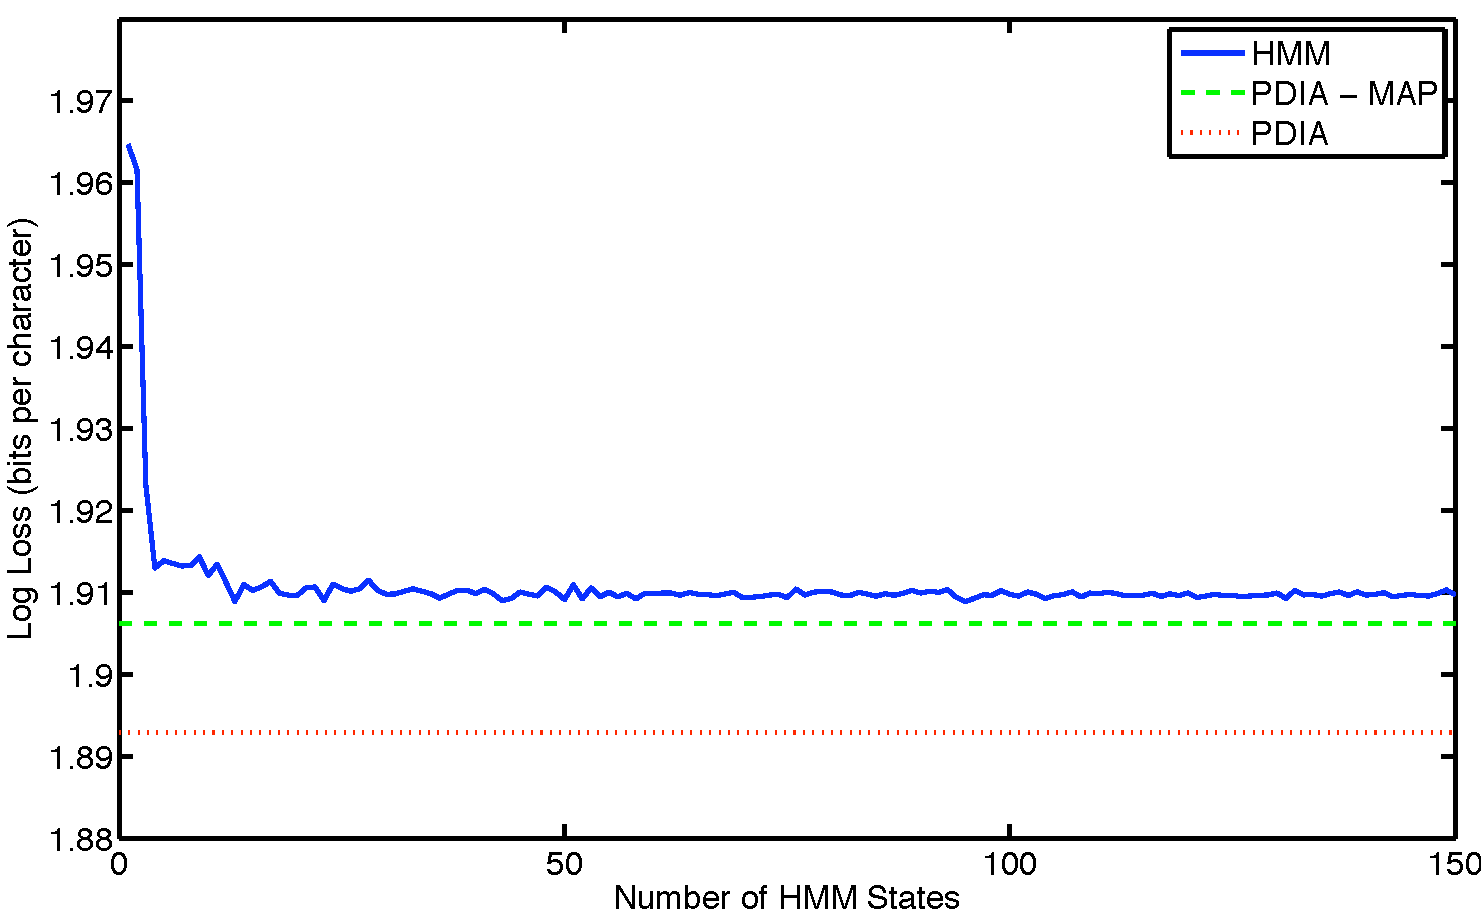
\includegraphics[width=.5\textwidth]{results/dna_hmm}
\caption{DNA HMM EM Baseline}
\label{fig:dna_hmm}
\end{center}
\end{figure}

\begin{figure}[htbp]
\begin{center}
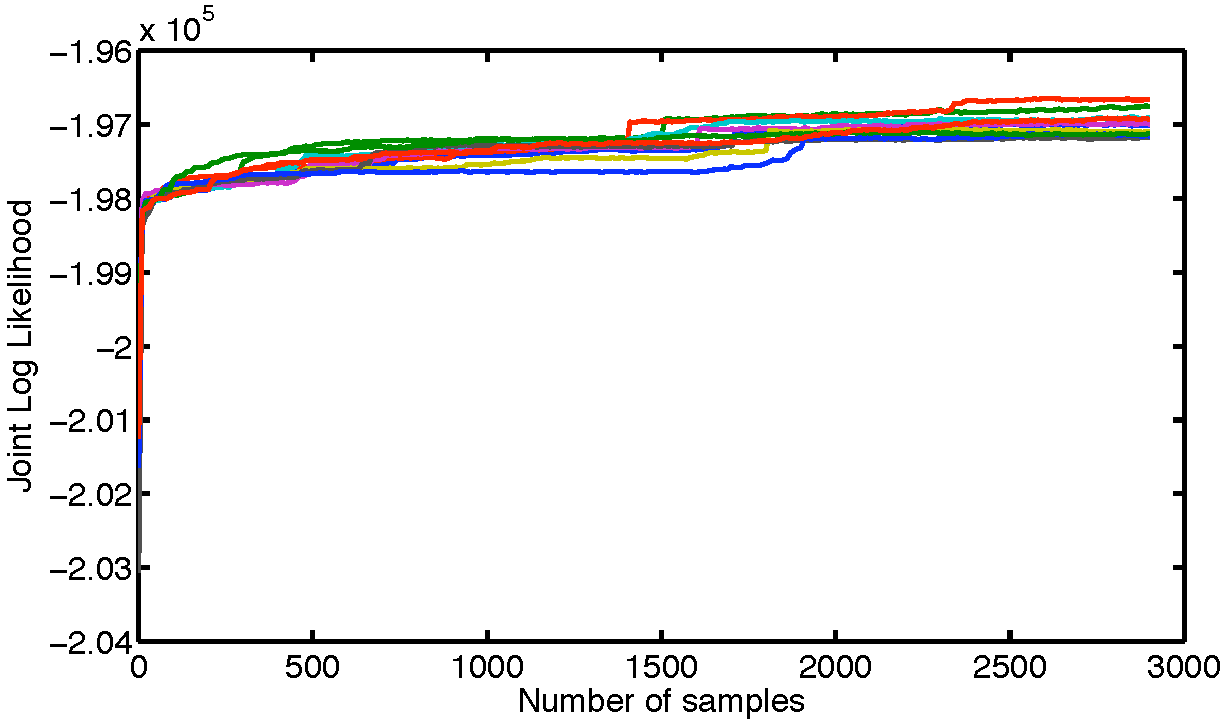
\includegraphics[width=.5\textwidth]{results/dna_sampler}
\caption{DNA sampler trace }
\label{fig:dna_sampler}
\end{center}
\end{figure}

\begin{figure}[htbp]
\begin{center}
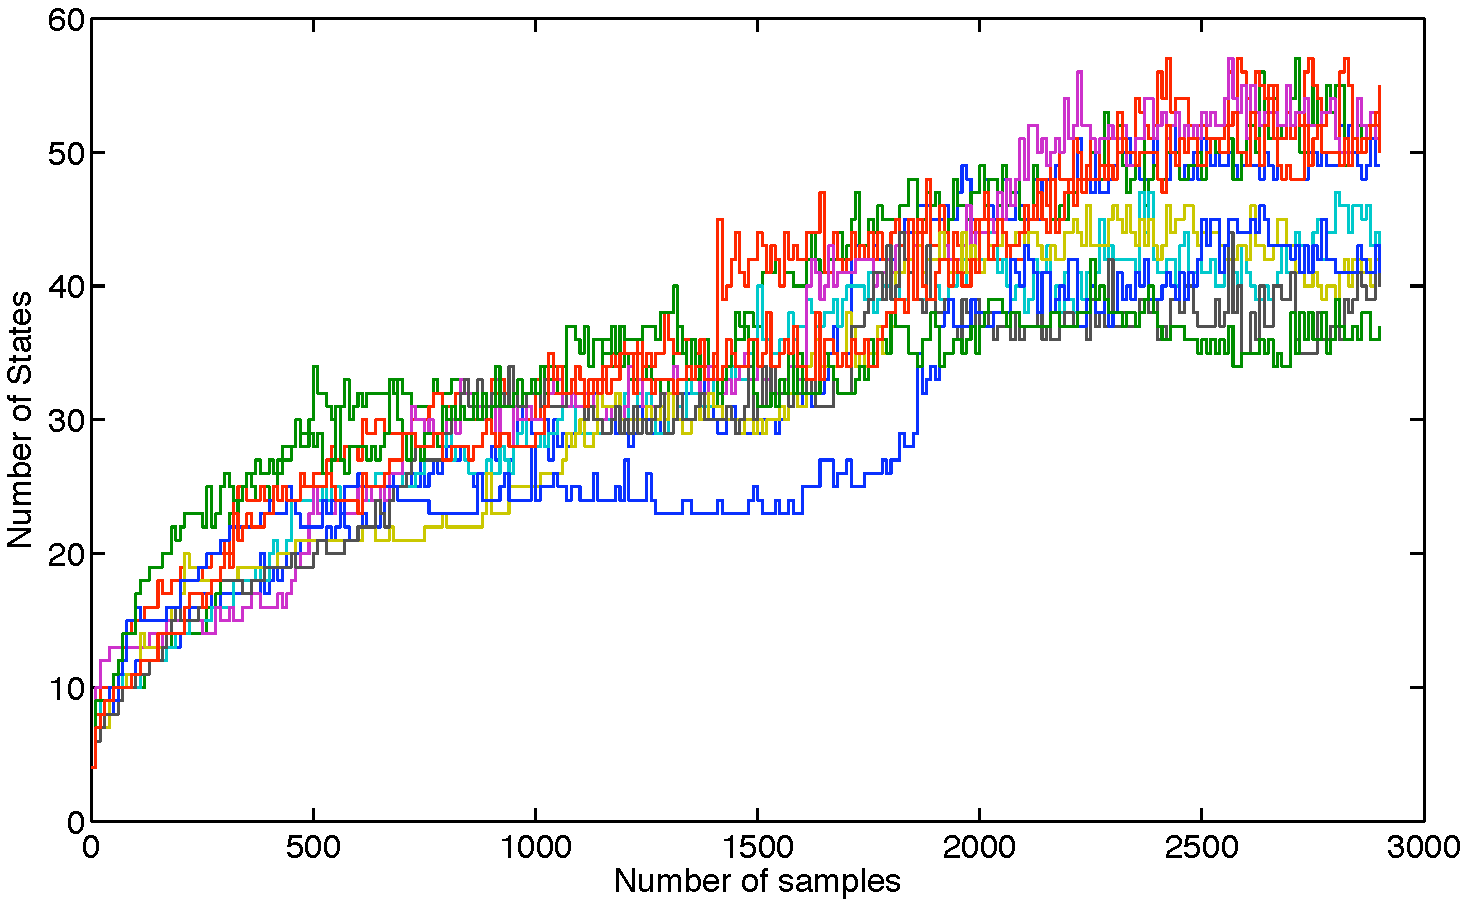
\includegraphics[width=.5\textwidth]{results/dna_numstates}
\caption{DNA number of states}
\label{fig:dna_numstates}
\end{center}
\end{figure}

\begin{figure}[htbp]
\begin{center}
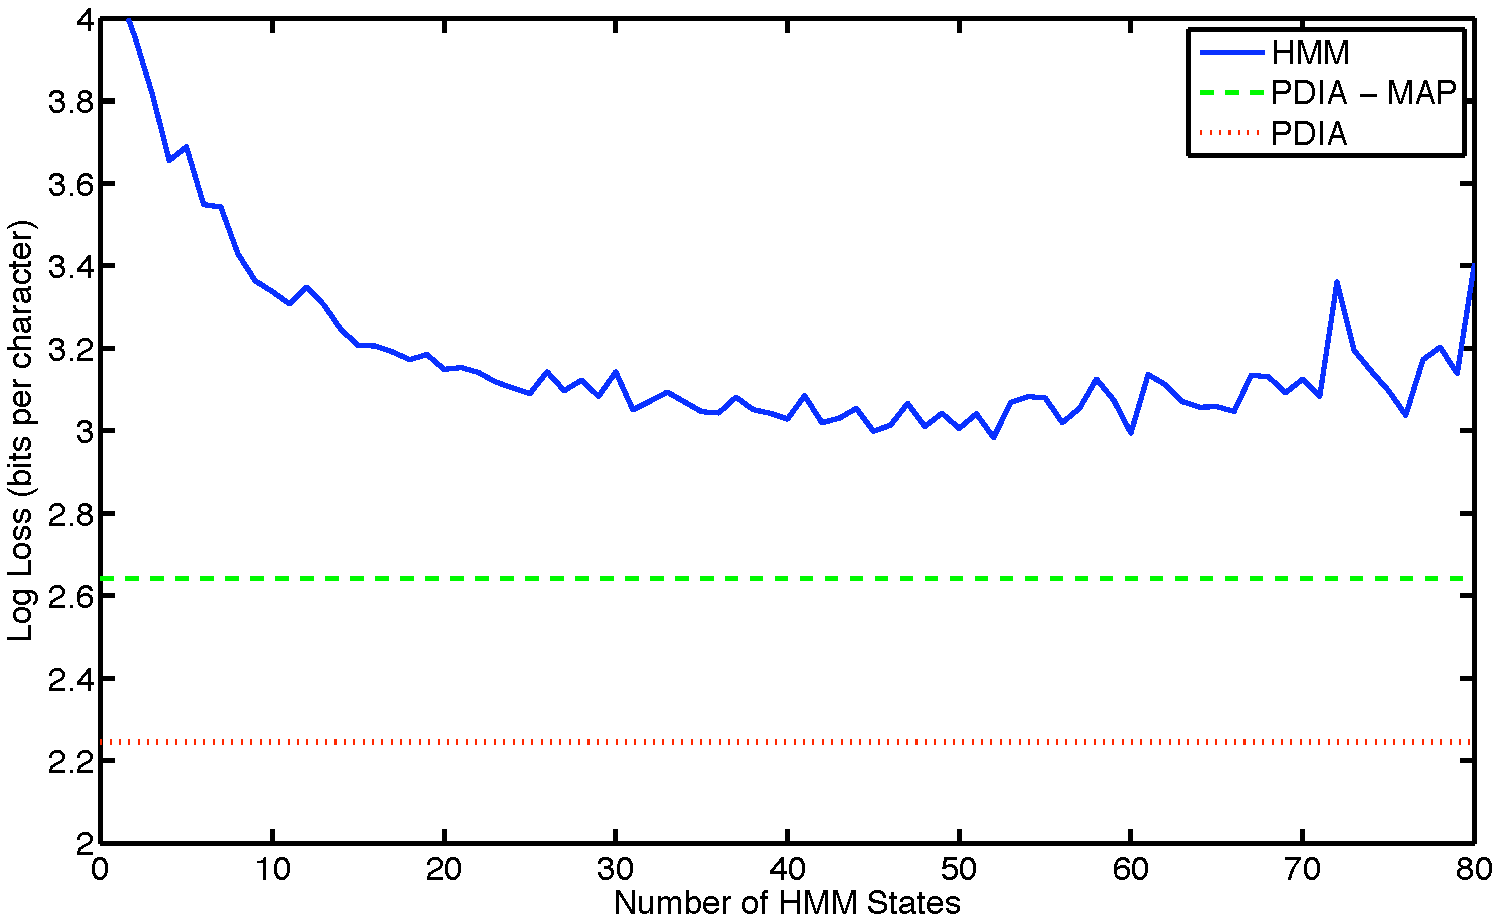
\includegraphics[width=.5\textwidth]{results/aiw_small_hmm}
\caption{AIW HMM EM Baseline}
\label{fig:aiw_small_hmm}
\end{center}
\end{figure}

\begin{figure}[htbp]
\begin{center}
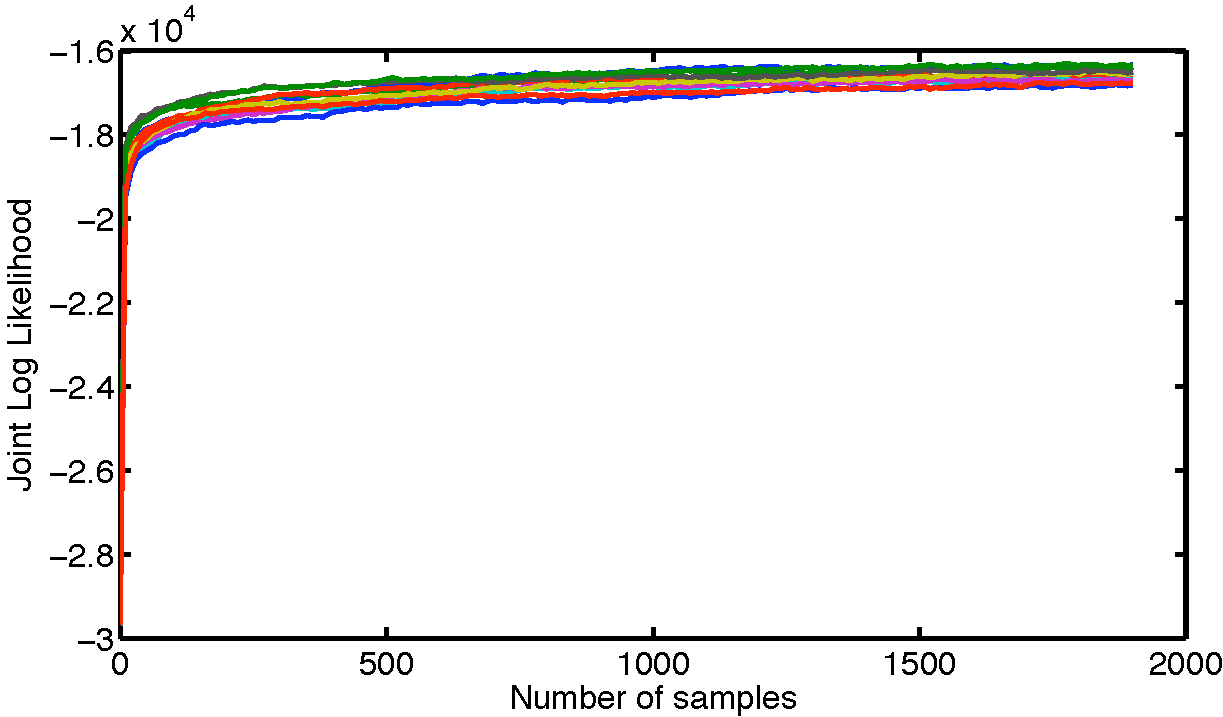
\includegraphics[width=.5\textwidth]{results/aiw_small_sampler}
\caption{AIW small sampler trace }
\label{fig:aiw_small_sampler}
\end{center}
\end{figure}

\begin{figure}[htbp]
\begin{center}
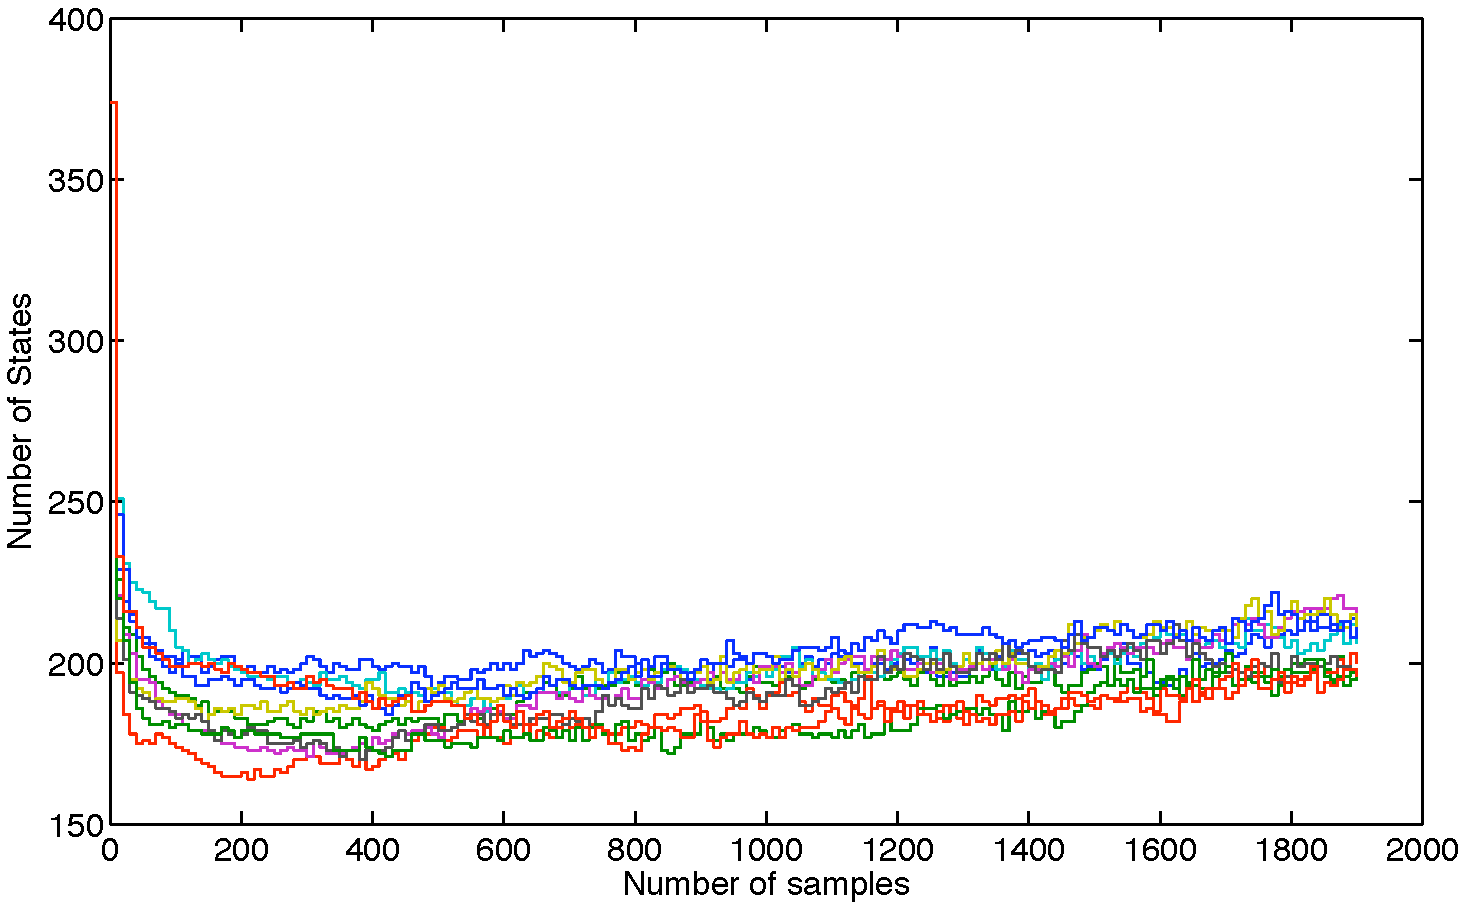
\includegraphics[width=.5\textwidth]{results/aiw_small_numstates}
\caption{AIW number of states}
\label{fig:aiw_small_numstates}
\end{center}
\end{figure}

We found that posterior samples from the PDIA achieve competitive generalization performance on natural language and DNA compared to hidden Markov models and n-gram models.  Averaging predictive probability over multiple samples leads to better generalization than a single sampled model.  Both a single sample and multiple samples generalize better than the best EM-trained HMM.  On natural language, the learned PDIA has more states than the optimal number of states for an HMM found by cross-validation.  The improved generalization is not due to smoothing the emission distribution.  Compared to smoothed n-gram models, the PDIA performs competitively even though there is no backing off to more general contexts.

We ran the PDIA on two datasets: Alice in Wonderland and mouse DNA.  Alice in Wonderland was preprocessed to remove all characters but letters and spaces, shift upper case to lower case, and split along sentence dividers to yield a 27-character alphabet (a-z and space) and 1639 sentences with a total of 132794 characters.  We used the first 1200 sentences (100210 characters) to train the model and the rest to test.  For some experiments we also used a smaller subset of Alice in Wonderland consisting of 100 randomly chosen training sentences (9986 characters) and 50 random test sentences (3891 characters).  The mouse DNA dataset consists of a fragment of chromosome 2 with 194173 base pairs, which we treated as a single unbroken string.  We used the first 150000 base pairs for training and the rest for testing.  For Alice in Wonderland, the state of the model was always set to $q_0$ at the start of a string.  For DNA, the state of the model at the start of the test data was set to the last state of the model after accepting the training data.  We placed Gamma(1,1) priors over $\alpha$,$\beta$ and $\gamma$ (what do we use for $\lambda$?) and saved every tenth MCMC sample for evaluating generalization.

To check the performance of our sampler, we trained it on data from three synthetic grammars: the even process \cite{?}, the Reber grammar \cite{Reber} and the Feldman grammar \cite{Feldman}, which have up to 7 states and 7 symbols in the alphabet.  Performance was good, even on small data.  Details are given in the appendix.

We evaluated the performance of the learned models by calculating the log loss per character of the test data.  For training data $x_{1:T}$, test data $y_{1:T'}$, and posterior samples $\boldsymbol\delta$, this is given by $-\frac{1}{T'}$log$_2\, P(y_{1:T'}|x_{1:T},\boldsymbol\delta)$.  It is a measure of the uncertainty of a character given the model, and is at most log$_2\,|\Sigma|$, which for DNA is 2 and for text is 4.755.  We evaluated the probability of the test data incrementally, and averaged each probability over multiple posterior samples: $P(y_{1:T'}|x_{1:T},\boldsymbol\delta) = \prod_{i = 1}^{T'} P(y_i|y_{1:i-1},x_{1:T},\boldsymbol\delta) = \frac{1}{L}\prod_{i = 1}^{T'} \sum_{\ell = 1}^{L} P(y_i|y_{1:i-1},x_{1:T},\delta_\ell)$.  In addition to averaging over multiple $\delta_\ell$, we also evaluated the log loss for each $\delta_\ell$ by itself to find the single model with the best generalization performance, which we call $\delta_{MAP}$.

Even for a single sampled transition matrix $\delta_\ell$, there may be symbols $y_t$ which have not been emitted from the state $\q_t$ in the training data, and thus $\delta_\ell(\q_t,y_t)$ is not known.  In this case we sampled a new element of the transition matrix according to the CRF, as described in \ref{model}.  In the same way that we averaged the predictive probability of each character over multiple $\delta_\ell$, we averaged the probability of a character given a single $\delta_\ell$ over multiple sampled values of $\delta_\ell(\q_t,y_t)$.

For a baseline result to compare our model against, we used two models: a hidden Markov model (HMM) and a smoothed n-gram model.  We used Kevin Murphy's HMM toolbox \cite{Murphy} and trained the HMM using expectation-maximization (EM).  We found the best number of hidden states by cross-validation on the same test data used for the PDIA.  The log loss and optimal number of states are given in Table \ref{table:results}, and plots showing the generalization performance across a range of model sizes relative to PDIA performance is given in Figures \ref{fig:dna_hmm} and \ref{fig:aiw_small_hmm}.  

We found that both the MAP PDIA and the average over PDIA generalize better than the HMM.  To test the possibility that better generalization was due to smoothing of the PDIA emission probability by $\beta$, we took samples from the PDIA, fixed $\beta$ to be very near 0, and ran the MCMC sampler as before.  We found that neither the average number of states nor the generalization performance was significantly affected.

For the smoothed n-gram model, we used a hierarchical Pitman-Yor Process language model (HPYPLM) \cite{Teh}, a hierarchical nonparametric Bayesian generalization of Kneser-Ney smoothing.  While the PDIA learns a larger class of models than an $n$-gram model, the emission probabilities of an HPYPLM are tied together in a more intelligent way than those of the PDIA, such that states with few observations still generalize well.  We ran the HPYPLM with Markov order 1 through 5 (that is, 2-gram through 6-gram).  We also evaluated the performance of the sequence memoizer (SM), which is the limit of an $n$-gram as $n\rightarrow\infty$.
